\chapter{Preliminary Graph Theory}\label{ch:prelim}

First, let's define some basic concepts of graph theory, starting with the graph itself.

\section{Graphs}

A graph is an algebraic structure most commonly used to describe relationships between objects. There are many definitions of a graph, the most abstract being simply a set $V$ and a relation $R$ on $V$ denoting which elements of $V$ are connected. Graphs in general are \textit{directed}; if $R$ is symmetric, the graph is \textit{undirected}. For the purposes of this work we will be using a geometric definition and generally undirected graphs.
An undirected graph is an ordered pair $G = (V, E)$, where $V$ is a set of \textit{vertices} and $E$ is a set of \textit{edges}, determining the incidence of vertices.

$$(\forall e \in E) ~ e = uv = vu; u,v \in V$$

A \textit{path} in a graph $G$ from $v$ to $w$; $v,w \in V$ is a sequence of vertices $(u_1, u_2, \dots, u_n); ~ \{u_i ~|~ 1 \leq i \leq n\} \subseteq V$ such that $u_1 = v$, $u_n = w$ and $\{(u_i, u_{i+1}) ~|~ 1 \leq i \leq n-1\} \subseteq E$. A graph is \textit{connected} if there exists a path between every pair of vertices $v,w \in V; ~ v \neq w$.
A \textit{degree} $\Delta (v)$ of a vertex $v$ denotes how many edges are incident to this vertex. The highest degree of any vertex in $G$ is denoted as $\Delta(G)$.
A graph is \textit{k-regular} if the degree of each vertex is exactly $k$. A \textit{cubic graph} is a 3-regular graph.

As an example, the smallest cubic graph is a complete graph with 4 vertices $K_4$. (In a complete graph each vertex is incident with each other vertex.).

\begin{figure}[h]
    \centering
        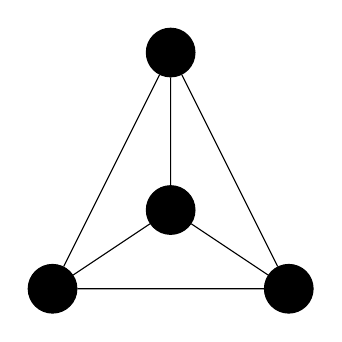
\begin{tikzpicture}
            \begin{scope}[every node/.style={circle,draw,fill=black}]
                \node (1) at (0,0) {1};
                \node (2) at (0,2) {2};
                \node (3) at (-1.5,-1) {3};
                \node (4) at (1.5,-1) {4};
            \end{scope}
            \draw (1) -- (2) -- (3) -- (4) -- (1) (2) -- (4) (1) -- (3);
        \end{tikzpicture}
        \caption[Smallest cubic graph]{Smallest cubic graph.}
\end{figure}

In general statements about graphs in later chapters we are referring to undirected cubic graphs.

We also need to define the set of \textit{half-edges} or vertex-edge incidences of a graph (or signed graph)

$$\Sigma _{G} = \bigcup _{e = vw \in E _{G}} \{(e, v), (e, w) \}$$

because in case of signed edge colouring we will be colouring half-edges instead.

\subsection{Colouring}

When simple binary relationships between objects are not enough, weighted graphs and colouring offer a wider range of applications. Assigning colours to vertices or edges of graphs makes classifications of these objects more robust.
A vertex colouring $\phi : V_G \rightarrow C$ of a graph $G$ is a mapping from the vertex set of $G$ to a set of colours $C$. An edge colouring $\chi : E_G \rightarrow C$ of a graph $G$ is a mapping from the edge set of $G$ to a set of colours $C$.
A \textit{proper vertex colouring} of $G$ is a vertex colouring such that no two incident vertices share a colour. A \textit{proper edge colouring} is an edge colouring such that no two incident edges have the same colour. A proper colouring using $k$ colours is called a \textit{$k$-colouring}.

As colouring in general is not very interesting, we will be considering only proper colourings henceforth. It is also important to define the set of "colours", especially when colouring signed graphs. It is most practical to use a subset of integers $C \subseteq \mathbb{Z}$ because it makes definitions and proofs clear. Additionally, it is important that a $k$-colouring uses a set of $k$ colours.

The typical colouring problem is to find the minimum number of colours required for a proper colouring. This number is called the \textit{chromatic number} for vertex colourings and \textit{chromatic index} for edge colourings. Determining the chromatic number and index is useful in other areas of graph theory as well.

\begin{theorem}\label{th:bipartite}
    A graph is bipartite if and only if it has a proper vertex 2-colouring.
\end{theorem}

For unsigned graphs these numbers are known.

\begin{theorem}[Brooks \cite{brooks}]
    The chromatic number of a connected graph $G$ is $\Delta(G)$ for all graphs except complete graphs and cycles of odd length, where the chromatic number is $\Delta(G) + 1$.
\end{theorem}

\begin{theorem}[Vizing]
    The chromatic index of a simple graph $G$ is $\Delta(G)$ or $\Delta(G) + 1$.
\end{theorem}

In other words, we can always colour the edges of a graph using at most $\Delta(G) + 1$ colours. The lower bound $\Delta(G)$ is trivial; we need exactly $\Delta(G)$ colours at the highest degree vertex in $G$ to construct a proper colouring. The Vizing theorem proves the upper bound using Kempe chains.

\section{Signed graphs}

A \textit{signed graph} $\Gamma = (G, \sigma)$ consists of an \textit{underlying graph} $G$ and a \textit{sign function} $\sigma : E(G) \rightarrow \{+,-\}$ that assigns a sign ($+$ or $-$) to each edge of $G$. $\Gamma ^+ = (V _{\Gamma}, E _{\Gamma ^+})$ and $\Gamma ^- = (V _{\Gamma}, E _{\Gamma ^-})$ denote subgraphs of $\Gamma$ with positive and negative edges respectively, $E _{\Gamma ^+} = \sigma ^{-1} (+1)$ and $E _{\Gamma ^-} = \sigma ^{-1} (-1)$. $\mathcal{S} (G)$ denotes the set of all signed graphs with the underlying graph $G$.

\begin{figure}[h]
    \centering
        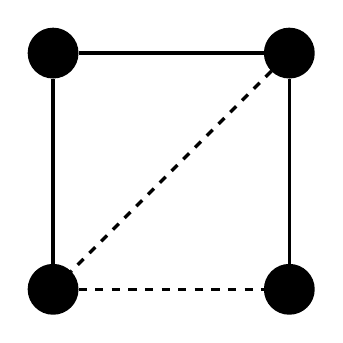
\begin{tikzpicture}
            \begin{scope}[every node/.style={circle,thick,draw,fill=black}]
                \node (1) at (0,0) {1};
                \node (2) at (3,0) {2};
                \node (3) at (0,-3) {3};
                \node (4) at (3,-3) {4};
            \end{scope}
            \begin{scope}[every edge/.style={draw,very thick}]
                \path
                    (1) edge (2)
                    (2) edge [dashed] (3)
                    (3) edge (1)
                    (2) edge (4)
                    (3) edge [dashed] (4);
            \end{scope}
        \end{tikzpicture}
    \caption[Example of a signed graph]{Example of a signed graph. Dashed edges are negative, solid edges are positive.}
\end{figure}

A fundamental concept in the theory of signed graphs is \textit{vertex switching}. Switching vertex $v$ of a signed graph reverses the sign of each edge incident with $v$. More generally, switching a signed subgraph reverses the sign of each edge between a vertex subset and its complement. Let's define switching by a \textit{switching function}

$$\theta : V_{\Gamma} \rightarrow \{+1, -1\}$$

where vertices mapped to $-1$ are being switched. The new graph will have an altered sign function,

$$\Gamma ^{\theta} = (G, \sigma ^{\theta}); ~~ \sigma ^{\theta} (uv) = \theta (u) \sigma (uv) \theta (v)$$

If a signed graph can be obtained from another signed graph by switching, they are considered \textit{switching equivalent}. Switching equivalence is an equivalence relation and thus forms equivalence classes on $\mathcal{S} (G)$. It makes sense to study properties of signed graphs that behave consistently under switching. An example of such a property is the signs of cycles. Switching doesn't change the sign of cycles because if a switched vertex is a part of a cycle, it will reverse the sign of two edges on that cycle leaving the sign product the same. In fact, the sign (or balance, defined below) of cycles is an alternative definition of a switching equivalence class, each combination of balance among a set of cycles that form a cycle space basis yields the same equivalence classes as the method used in this thesis and defined later. It is also important to point out that switching a set of vertices is equivalent to a sequence of one-vertex switches.

Directly related to vertex switching is the notion of \textit{balance}. A cycle is \textit{balanced} when the product of signs of its edges is positive and \textit{unbalanced} otherwise. A signed graph $\Gamma$ is balanced when each cycle in $\Gamma$ is balanced. It is \textit{antibalanced} if each cycle is unbalanced. Note that balanced doesn't imply \textit{all-positive}, there are balanced graphs with negative edges (see \cref{fig:balanced}).

\begin{theorem}[Harary \cite{harary}]\label{th:harary}
    A signed graph is balanced if and only if
    \begin{enumerate}
        \item for every pair of vertices, all paths between these vertices have the same sign
        \item the vertices can be divided into two subsets (possibly empty) such that each edge with both ends in the same subset is positive and each edge with ends in different subsets is negative
    \end{enumerate}

    This is a generalization of the earlier mentioned bipartite graph theorem (\Cref{th:bipartite}).
\end{theorem}

\begin{figure}[h]\label{fig:balanced}
    \centering
    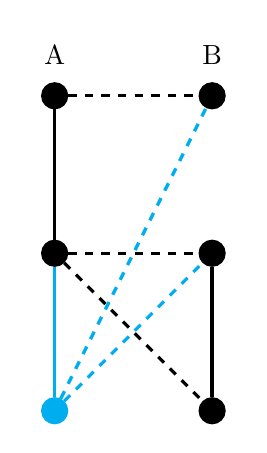
\begin{tikzpicture}
        \begin{scope}[every node/.style={circle,draw,fill=black}]
            \node (1) [fill=cyan,color=cyan] at (0,0) {};
            \node (2) at (0,2) {};
            \node (3) [label=above:A] at (0,4) {};
            \node (5) at (2,0) {};
            \node (6) at (2,2) {};
            \node (7) [label=above:B] at (2,4) {};
        \end{scope}
        \begin{scope}[every edge/.style={draw,very thick}]
            \path
                (1) edge [color=cyan] (2)
                (3) edge (2)
                (5) edge (6)
                (2) edge [dashed] (5)
                (2) edge [dashed] (6)
                (3) edge [dashed] (7)
                (1) edge [dashed,color=cyan] (7)
                (1) edge [dashed,color=cyan] (6);
        \end{scope}
    \end{tikzpicture}
    \hspace{0.1\textwidth}
    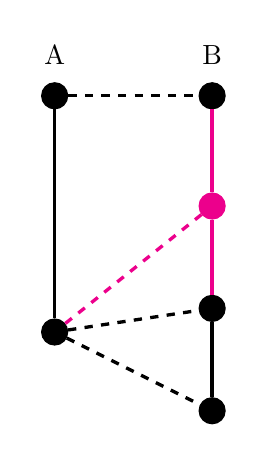
\begin{tikzpicture}
        \begin{scope}[every node/.style={circle,draw,fill=black}]
            \node (1) [fill=magenta,color=magenta] at (2,2.6) {};
            \node (2) at (0,1) {};
            \node (3) [label=above:A] at (0,4) {};
            \node (5) at (2,0) {};
            \node (6) at (2,1.3) {};
            \node (7) [label=above:B] at (2,4) {};
        \end{scope}
        \begin{scope}[every edge/.style={draw,very thick}]
            \path
                (1) edge [dashed,color=magenta] (2)
                (1) edge [color=magenta] (6)
                (5) edge (6)
                (3) edge (2)
                (2) edge [dashed] (5)
                (2) edge [dashed] (6)
                (3) edge [dashed] (7)
                (1) edge [color=magenta] (7);
        \end{scope}
    \end{tikzpicture}
    \caption[Switching a balanced graph]{Switching a balanced graph.}
\end{figure}

An all-positive graph $\Gamma$ is trivially balanced, all paths are positive and the division of vertices will be subsets $V_{\Gamma}$ and $\emptyset$. Only graphs switching equivalent to an all-positive graph are balanced. Consider how the conditions in \cref*{th:harary} behave under switching.

Let's say we switch vertex $v \in V_{\Gamma}$. The sign of each path that ends at $v$ from any other vertex will flip, because exactly one edge on that path changed signs. So if all paths between $v$ and any other vertex, say $u$, had the same sign before switching, now they will have the opposite but still the same sign.

Suppose we are able to divide $V_{\Gamma}$ into two subsets $A$ and $B$ as per the second condition in \cref*{th:harary} and without loss of generality let $v \in A$. So all edges $vx; ~ x \in A$ are positive and all edges $vy; ~ y \in B$ are negative. After switching $v$ we will construct a new division of $V_{\Gamma}$, subsets $A' = A \setminus \{v\}$ and $B' = B \cup \{v\}$. $A'$ and $B'$ is obviously a correct division of $V_{\Gamma}$ and the second condition will still hold, since all edges incident with $v$ flipped signs and at the same time changes whether they end in the same sunbset as $v$ or not.

Connected to vertex switching is the notion of \textit{balance}. The sign of a path is the product of the signs of its edges. A path is positive if and only if there is an even number of negative edges on it. A cycle is balanced if it is positive and a signed graph is balanced if each cycle in it is balanced\cite{harary}.

\subsection{Colouring}

The research of signed graph colouring was initiated by Zaslavsky\cite{zaslavsky-graphs} in the early 1980s and published in multiple seminal papers \cite{zaslavsky-invariants,zaslavsky-colouring,zaslavsky-colourful}. Before defining signed vertex and edge colouring it is necessary to define the set of colours.

In the context of signed graphs and vertex switching we are looking for a set of signed integers with the idea of switching a color reversing its sign, same operation as with the signs of edges. Proper colourings of signed graphs will then be consistent under vertex switching because "reversing the sign" is a bijection on $\mathbb{Z}$. Zaslavsky \cite{zaslavsky-colouring} defined a $k$-colouring based on a signed colour set $C_k = \{-k, -(k-1), \dots, -1, 0, 1, \dots, (k-1), k\}$ and called colourings zero-free if the colour $0$ was not used. He then studied the properties of \textit{chromatic polynomials} related to signed colourings, the number of colourings for a signed graph. (Balanced chromatic polynomials in case of zero-free colourings.)

However, this definition is not a natural extension of the original colour set of integers, because a $k$-colouring essentially uses $2k$ or $2k+1$ signed colours. This is a desirable property for the colour set, since signed graphs themselves are an extension of unsigned graphs the signed color set should behave in a similar way. A balanced signed graph is essentially equivalent to the unsigned underlying graph, so its chromatic number and index for instance should also match. Máčajová et al. offer another definition: a $k$-colouring uses the colour set $C_k = \{\pm 1,\pm 2,\dots,\pm k\}$ if $n = 2k$ and $C_k = \{0, \pm 1,\pm 2,\dots,\pm k\}$ if $n = 2k + 1$. Behr \cite{behr-edge-colouring} also adopts this definition.

A vertex colouring $\phi : V_{\Gamma} \rightarrow C_k$ of a signed graph $\Gamma$ is, similarly to unsigned graphs, a mapping from the vertex set of $\Gamma$ to a set of signed colours $C_k$.

Edge colouring, however, needs to be defined differently to incorporate the additional information given by the edge signs. The definition of a $k$-coloring $\gamma : \Sigma _{\Gamma} \rightarrow C_k$ of a signed graph $\Gamma$ inspired by Behr \cite{behr-edge-colouring} is a mapping from the set of half-edges of $\Gamma$ to a set of signed colours $C_k$ such that

$$(\forall e = uv \in E_{\Gamma}) ~~ \gamma(e, u) = \sigma(e)\gamma(e, v)$$

In other words, half-edges that form a positive edge must have the same color and half-edges that form a negative edge must have opposite colors. The only difference to Behr's version is the usage of $\sigma(e)$ instead of $-\sigma(e)$, which is really only a matter of taste. In our version positive edges behave like unsigned instead of negative which seemed more natural. Between these definitions different signatures are colorable, but they are equivalent in the sense that there is a bijection between graphs colorable under our definition and Behr's definition. If signed graph $\Gamma = (G, \sigma)$ is edge colorable under our definition, then $\Gamma' = (G, -\sigma)$ with the sign of each edge reversed is colorable under Behr's.

An edge coloring of a signed graph is \textit{proper} if, just as with unsigned graphs, each color is present at each vertex at most once. In case of a vertex coloring all neighbors of each vertex must have different colors. We will, again, consider only proper colorings from now on.

\begin{figure}[h]
    \centering
    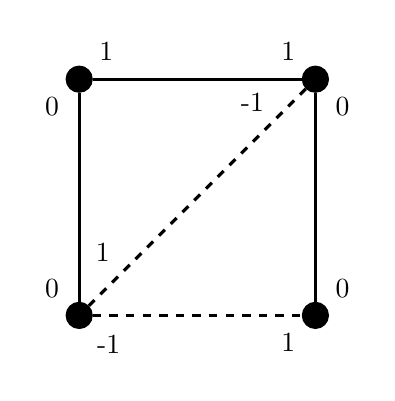
\begin{tikzpicture}
        \begin{scope}[every node/.style={circle,draw,fill=black}]
            \node (1) [label=above right:1, label=below left:0] at (0,0) {};
            \node (2) [label=above left:1, label=below right:0] at (3,0) {};
            \node (3) [label=above left:0, label=below right:-1] at (0,-3) {};
            \node (4) [label=above right:0, label=below left:1] at (3,-3) {};
        \end{scope}
        \node (ar) at (2.2,-0.3) {-1};
        \node (bl) at (0.3, -2.2) {1};
        \begin{scope}[every edge/.style={draw,very thick}]
            \path
                (1) edge (2)
                (2) edge [dashed] (3)
                (3) edge (1)
                (2) edge (4)
                (3) edge [dashed] (4);
        \end{scope}
    \end{tikzpicture}
    \hspace{0.1\textwidth}
    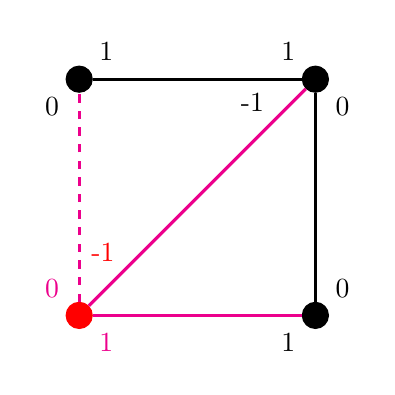
\begin{tikzpicture}
        \begin{scope}[every node/.style={circle,draw,fill=black}]
            \node (1) [label=above right:1, label=below left:0] at (0,0) {};
            \node (2) [label=above left:1, label=below right:0] at (3,0) {};
            \node (3) [label={[text=magenta]above left:0}, label={[text=magenta]below right:1},red] at (0,-3) {};
            \node (4) [label=above right:0, label=below left:1] at (3,-3) {};
        \end{scope}
        \node (ar) at (2.2,-0.3) {-1};
        \node (bl) [red] at (0.3, -2.2) {-1};
        \begin{scope}[every edge/.style={draw,very thick}]
            \path
                (1) edge (2)
                (2) edge [magenta] (3)
                (3) edge [dashed,magenta] (1)
                (2) edge (4)
                (3) edge [magenta] (4);
        \end{scope}
    \end{tikzpicture}
    \caption[Example of a signed edge coloring]{Example of a proper signed edge coloring on the left. We obtain the graph on the right by switching the bottom left vertex and the coloring remains correct and proper.}
\end{figure}

\section{Motivation}

Behr proved a signed version of the Vizing's theorem.

\begin{theorem}[Signed Vizing's theorem \cite{behr-edge-colouring}]
    The chromatic index of a simple \textit{signed} graph $\Gamma$ is $\Delta(\Gamma)$ or $\Delta(\Gamma) + 1$.
\end{theorem}

This opens the door for research into edge 3-coloring and cubic signed snarks.

\say{In the study of various important and difficult problems in graph theory (such as the cycle double cover conjecture and the 5-flow conjecture), one encounters an interesting but somewhat mysterious variety of graphs called snarks. In spite of their simple definition [\dots] and over a century long investigation, their properties and structure are largely unknown.} --- Chladný, Škoviera \cite{skoviera-citat}

The exact definition of a snark may vary from paper to paper but a snark is essentially a cubic graph with chromatic index four (its edges can't be coloured with three colours). Every cubic graph with a loop or a bridge is trivially a snark, triangles (cycles of length three) can be contracted into a single vertex and cycles of length four can also be simplified. Therefore many definitions forbid these properties by considering true snarks only graphs with girth (length of the shortest cycle) at least five. Even stronger, sometimes only cyclically 4-edge-connected graphs are considered (there is no subset of three or fewer edges such that their removal will disconnect the graph into two subgraphs each containing a cycle). One of the alternative formulations of the four colour theorem is that each snark is non-planar.

Signed snarks, however, are not subject to the same trivial cases or reductions. For instance, signed graphs with loops or bridges might have colorable signatures and only balanced triangles can be contracted into one vertex. That is why we will be considering any connected cubic signed graph with chromatic index 4 a \textit{signed snark}.

\section{Previous research}

Máčajová et al. expanded upon Zaslavsky's research by studying the properties of the chromatic number of signed graphs, ultimately proving a signed version of the famous Brooks' \cite{brooks} theorem.

\begin{theorem}[Signed Brooks' Theorem]\label{th:brooks}
    Let $\Gamma$ be a simple connected signed graph. If $\Gamma$ is not a balanced complete graph, a balanced odd circuit or an unbalanced even circuit, then $\chi(\Gamma) \leq \Delta(\Gamma)$.
\end{theorem}

In addition to the Signed Vizing's theorem Behr \cite{behr-edge-colouring} proved that there is a bijection between proper edge colorings of $\Gamma$ and proper vertex colorings of the negative of the line graph of $\Gamma$.
